\section{Durchführung}

Der Versuchsaufbau besteht aus einem Ultraschallechoskop mit drei verschiedenen Ultraschallsonden.
Die Sonden haben \SI{1}{\mega\hertz}, \SI{2}{\mega\hertz} und \SI{4}{\mega\hertz}.
Außerdem steht noch ein Rechner für die Datenaufnahme zur Verfügung.
Bei diesem Versuch wird nur das Impuls-Echo-Verfahren verwendet und die Leistung der
Sonden kann von $0-35 \, dB$ eingestellt werden.

In dem ersten Teil des Versuchs werden die Durchmesser von Bohrungen in einem Acrylblock
bestimmt. Der Block ist mit den Bohrungen in Abbildung (\ref{abb:1}) schematisch dargestellt.

\begin{figure}[H]
  \centering
  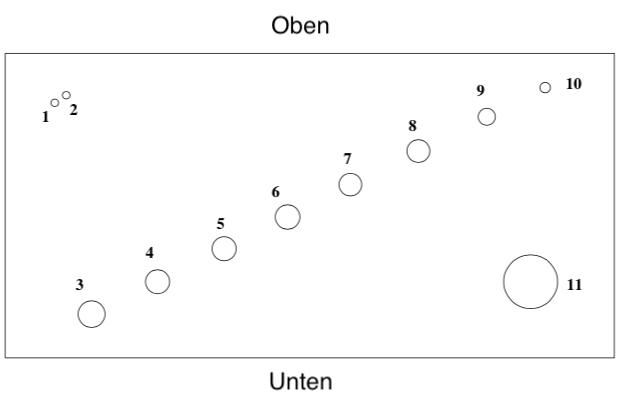
\includegraphics[width=\textwidth]{content/Block.png}
  \caption{Darstellung des Acrylblocks \cite{1}.}
  \label{abb:1}
\end{figure}

Zunächst wird der Block und die Bohrungen mit einer Schieblehre vermessen.
Daraufhin werden die Lagen der Bohrungen mit einem A-Scan bestimmt, indem von oben
und von unten ein Scan durchgeführt wird.
Als nächstes werden diese Bohrungen durch einen B-Scan bestimmt. Dieser muss auch von
oben und von unten durchgeführt werden um den Durchmesser der Löcher bestimmen zu können.

In dem zweiten Teil wird ein Herzmodell untersucht. Das Modell besitzt eine bewegliche
Membran, mit der das \enquote{Herzvolumen} verändert werden kann. Damit wird die
Herzfrequenz simuliert.
Mit einem Time-Motion Scan wird nun die Herzfrequenz $\nu_\text{Herz}$ gemessen. Dabei wird das Modell
mit Wasser gefüllt und die Ultraschallsonde wird so eingestellt, dass sie das Wasser gerade
berührt. Aus der Frequenz kann dann das Herzvolumen bestimmt werden mit der Formel:

\begin{equation}
  HZV = (EDS - EDV) \nu_\text{Herz}
  \label{eq:2}
\end{equation}

Dabei ist $EDS$ das endsystolische Volumen und $EDV$ das enddiastolische Volumen.
